% University Assignment Title Page 
% LaTeX Template
% Version 1.0 (27/12/12)
%
% This template has been downloaded from:
% http://www.LaTeXTemplates.com
%
% Original author:
% WikiBooks (http://en.wikibooks.org/wiki/LaTeX/Title_Creation)
%
% License:
% CC BY-NC-SA 3.0 (http://creativecommons.org/licenses/by-nc-sa/3.0/)
% 
% Instructions for using this template:
% This title page is capable of being compiled as is. This is not useful for 
% including it in another document. To do this, you have two options: 
%
% 1) Copy/paste everything between \begin{document} and \end{document} 
% starting at \begin{titlepage} and paste this into another LaTeX file where you 
% want your title page.
% OR
% 2) Remove everything outside the \begin{titlepage} and \end{titlepage} and 
% move this file to the same directory as the LaTeX file you wish to add it to. 
% Then add \input{./title_page_1.tex} to your LaTeX file where you want your
% title page.
%
%%%%%%%%%%%%%%%%%%%%%%%%%%%%%%%%%%%%%%%%%
%\title{Title page with logo}
%----------------------------------------------------------------------------------------
% PACKAGES AND OTHER DOCUMENT CONFIGURATIONS
%----------------------------------------------------------------------------------------
\documentclass[12pt]{article}
\usepackage{polski}
\usepackage[utf8]{inputenc}
\usepackage{amsmath}
\usepackage{mathtools}
\usepackage{hyperref}
\usepackage{tikz}
\tikzset{
heap/.style={
every node/.style={shape=rectangle,rounded corners, draw},
level 1/.style={sibling distance=30mm},
level 2/.style={sibling distance=10mm}
}
}
\usepackage{blkarray, bigstrut}
\usepackage{graphicx}
\usepackage[colorinlistoftodos]{todonotes}
\usepackage[left=2.5cm,top=3cm,right=2.5cm,bottom=3cm,bindingoffset=0.5cm]{geometry}
\usepackage{multicol}
\usepackage{afterpage}
\usepackage{array}
\usepackage{pgfplots}
\usepackage{listings}
\lstset{
  showstringspaces=false
basicstyle=\ttfamily,
columns=fullflexible,
frame=single,
breaklines=true,
postbreak=\mbox{\textcolor{red}{$\hookrightarrow$}\space},
escapeinside={(*@}{@*)},
}
\usepackage{tabularx}
\usepackage{listings}
\usepackage{dirtree}
\usepackage{caption}
\usepackage[section]{placeins}
\usepackage{amsfonts}
%\captionsetup[figure]{font=small,labelfont=small}
%\captionsetup[table]{font=small,labelfont=small}

\newcommand\blankpage{%
\null
\thispagestyle{empty}%
\addtocounter{page}{-1}%
\newpage}
\pgfplotsset{compat=1.15}
\setcounter{tocdepth}{3}
\setcounter{secnumdepth}{3}
\setlength{\marginparwidth}{2cm}
\begin{document}
\begin{titlepage}

\newcommand{\HRule}{\rule{\linewidth}{0.5mm}} % Defines a new command for the horizontal lines, change thickness here

\center % Center everything on the page
\vspace*{\fill}
%----------------------------------------------------------------------------------------
% HEADING SECTIONS
%----------------------------------------------------------------------------------------

\textsc{\LARGE Politechnika Wrocławska}\\[0.5cm] % Name of your university/college
\textsc{\Large Wydział Elektroniki}\\[1.5cm] % Major heading such as course name
\textsc{\large Inżynieria e-systemów - technologia Java}\\[0.5cm] % Minor heading such as course title

%----------------------------------------------------------------------------------------
% TITLE SECTION
%----------------------------------------------------------------------------------------

\HRule \\[0.4cm]
{ \huge \bfseries Aplikacja internetowa służąca do analizowania sentymentu na rynkach finansowych}\\[0.4cm] % Title of your document
\HRule \\[1.5cm]
%----------------------------------------------------------------------------------------
% AUTHOR SECTION
%----------------------------------------------------------------------------------------

\begin{minipage}[t]{0.4\textwidth}
\begin{flushleft} \large
\emph{Autorzy:}\\
Jakub Sokołowski 226080\\
Konrad Olszewski 238898\\
\end{flushleft}
\end{minipage}
~
\begin{minipage}[t]{0.5\textwidth}
\begin{flushright} \large
\emph{Prowadzący:} \\
Dr inż. Tomasz Walkowiak
\end{flushright}
\end{minipage}\\

% If you don't want a supervisor, uncomment the two lines below and remove the section above
%\Large \emph{Author:}\\
%John \textsc{Smith}\\[3cm] % Your name

%----------------------------------------------------------------------------------------
% DATE SECTION
%----------------------------------------------------------------------------------------
\vspace*{\fill}

{\large \today}\\[2cm] % Date, change the \today to a set date if you want to be precise
\end{titlepage}
\newpage
\tableofcontents
\newpage
\section{Cel projektu}
Celem projektu jest stworzenie aplikacji webowej umożliwiającej analizę sentymentu na rynkach finansowych.
Przez sentyment rozumiemy: opinie na temat sytuacji na rynku (uzyskiwane za pomocą analizy postów, artykułów oraz komentarzy).
\subsection{Sentyment na rynkach finansowych}
W finansach behawioralnych, ważnym wskaźnikiem pozwalającym na opisanie zachowanie inwestorów lub osób zainteresowanych rynkiem jest sentyment. Sentyment możemy ogólnie zdefiniować jako skłonność do spekulacji (podejmowania nadmiernego ryzyka) oraz system oczekiwań, co do przyszłego kursu danego instrumentu finansowego. W pracy \textit{"Investor Sentiment in the Stock Market"} Baker i Wurgler rozważają teoretyczne wpływy sentymentu na rynki oraz instrumenty finansowe. Zgodnie z obserwacjami autorów badania, instrumenty finansowe cechujące się zwiększoną zmiennością cen oraz skomplikowaną wyceną, charakteryzują się większą podatnością na sentyment.
\section{Wymagania i założenia projektu}
\subsection{Wymagania funkcjonalne}
\begin{enumerate}
  \item {Wizualizacja przebiegu czasowego ceny instrumentu, za pomocą wykresów "candlestick". Zdecydowaliśmy się wybrać wykresy typu świecowego, ponieważ uwzględniają one zmiany ceny w okresie. Każda ze świec pokazuje cenę maksymalną, minimalną, jak również cenę otwarcia oraz zamknięcia. Wypełnienie świec kolorem zagwarantuje poprawę czytelności oraz ułatwi dostrzeganie zmian.}
  \item {Wyświetlanie danych sentymentu z zadanego przedziału czasowego, filtrowanie i agregacja danych. Pozwoli to użytkownikowi na komfort przeglądania interesujących danych oraz możliwość dogłębnej analizy jedynie interesującego przedziału czasu.}
  \item {Umożliwienie użytkownikowi uzupełnienia luk w danych - z wykorzystaniem komputera użytkownika. Wprowadzenie funkcjonalności pozwoli na "samodoskonalenie" się systemu oraz sprawi, że narzędzie stanie się bardziej kompleksowe.}
  \item {Umożliwienie pobrania danych w różnych formatach. Wprowadzenie funkcjonalności pozwoli użytkownikowi na pobranie danych w potrzebnym formacie. Przewiduje się umożliwienie pobrania danych w takich formatach jak: JSON oraz CSV - z możliwością wyboru separatora.}
\end{enumerate}
  \clearpage
\subsection{Wymagania niefunkcjonalne}
\begin{enumerate}
  \item {System przewiduje maksymalną ilość użytkowników równocześnie korzystających z systemu na poziomie 100 osób.}
  \item {System okresowo (godziny nocne, z uwagi na mniejsze obciążenie serwera) generuje kopie zapasowe.}
  \item {System przewiduje współpracę jedynie z nowoczesnymi przeglądarkami internetowymi.}
\end{enumerate}
\subsection{Założenia}
Z uwagi na brak zaplecza finansowego podczas realizacji projektu, dane wykorzystane do analizy sentymentu pochodzą głównie z portali takich jak: Reddit oraz Twitter, a wybranymi instrumentami finansowymi są kryptowaluty - Bitcoin, Ethereum, Litecoin etc. Zgromadzone dane zostały otagowane przy wykorzystaniu przetwarzania języka naturalnego (z ang. \textit{Natural Language Processing}, NLP) w Pythonie, w bibliotece VADER - część \textit{Natural Language Toolkit}. Analizator każdemu wyrażeniu przypisuje wartość z przedziału $[0; 1]$, w zależności od wydźwięku podanej frazy (pozytywna, negatywna lub neutralna).
\newpage
\section{Architektura projektu}
\begin{figure}[h!]
  \centering
    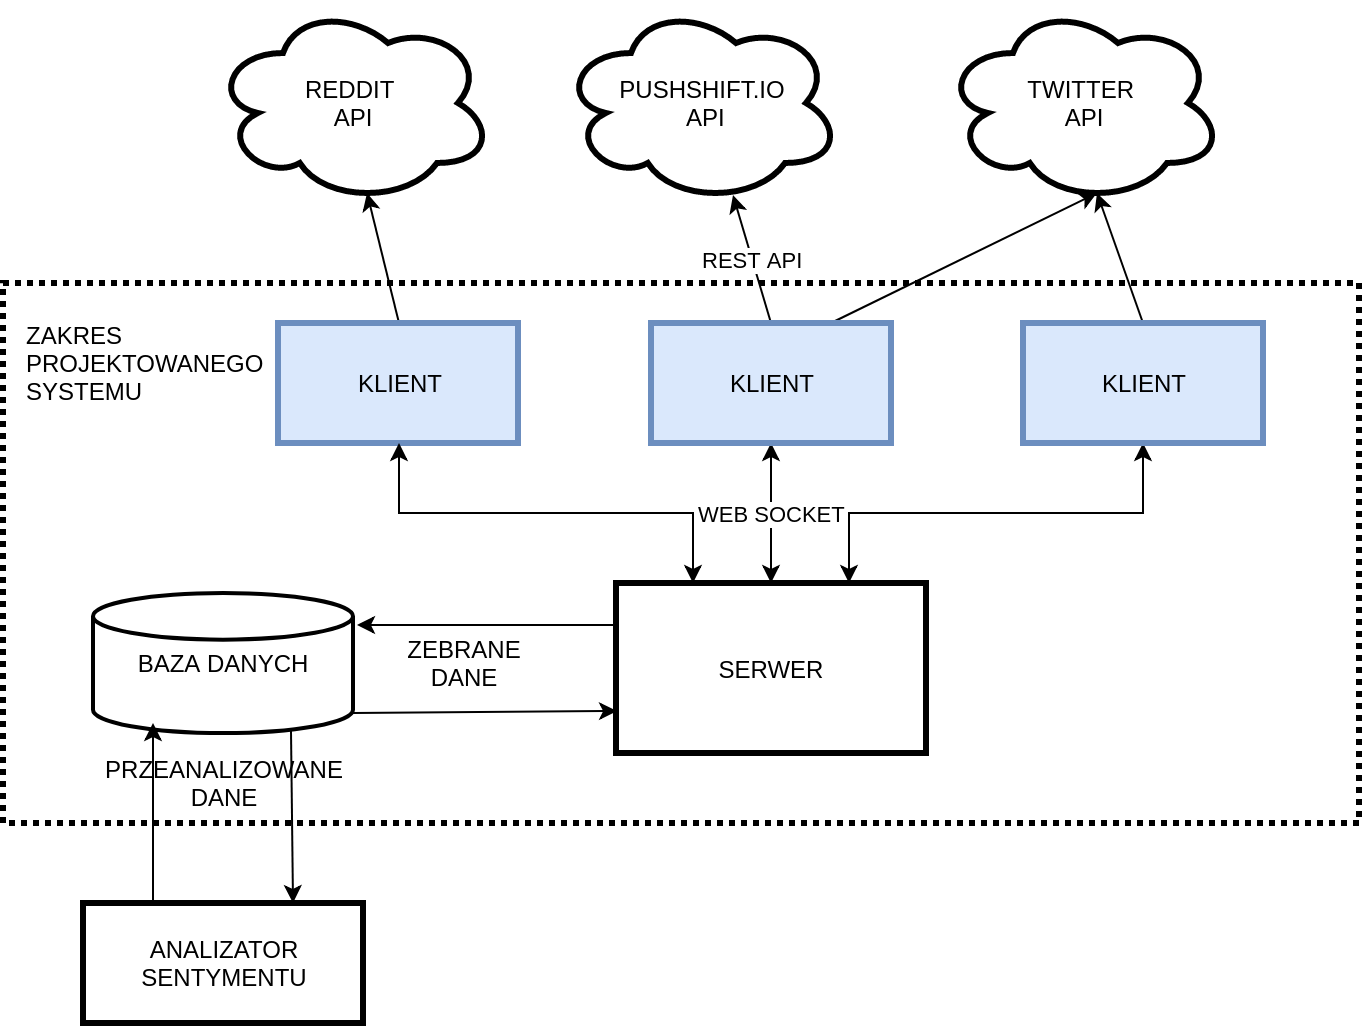
\includegraphics[width=0.95\textwidth]{img/architecture.png}
  \caption{Diagram architektury}
  \label{fig:arch}
\end{figure}
\newpage
\subsection{Model danych}
\subsection{Moduły}
\subsubsection{Serwer}
\begin{figure}[h!]
  \centering
    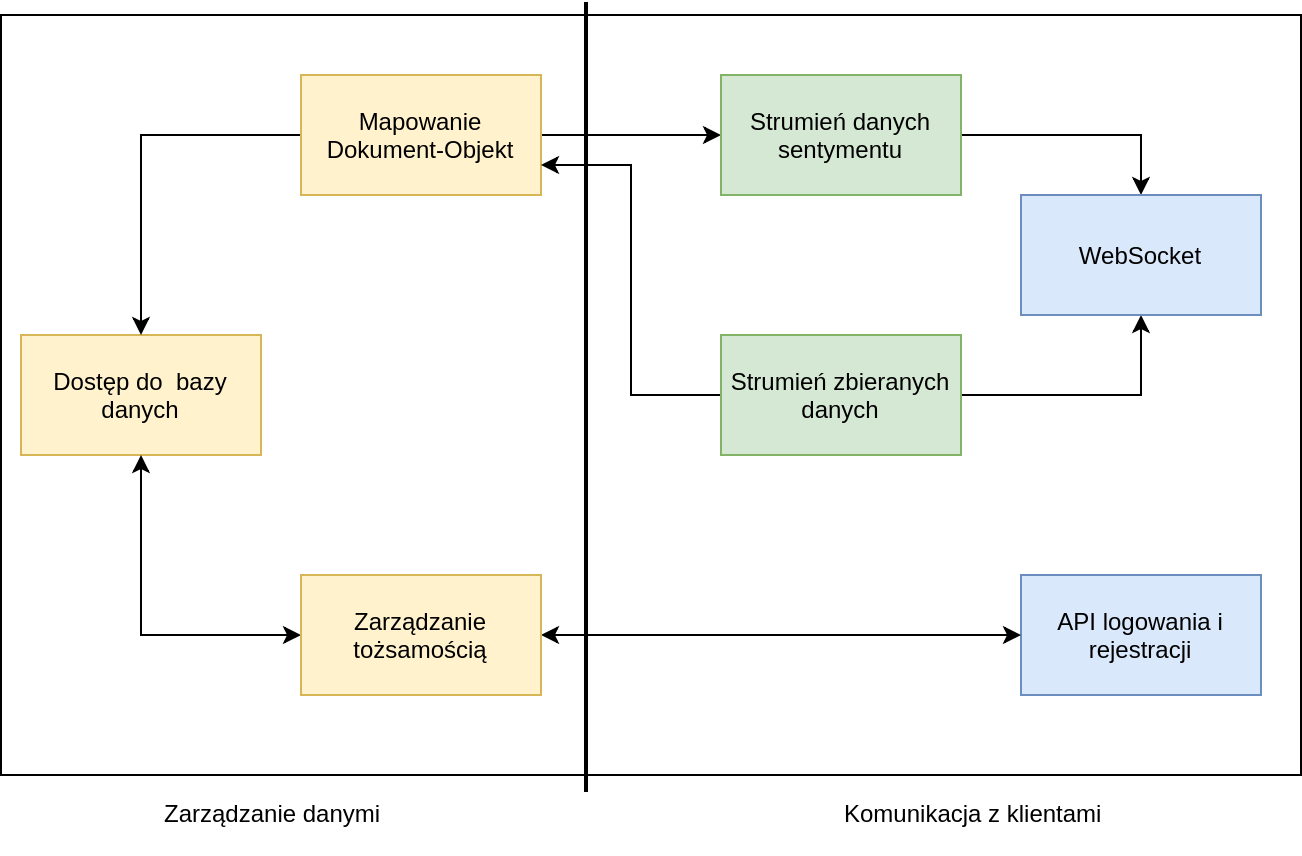
\includegraphics[width=0.95\textwidth]{img/serwer-modules.png}
  \caption{Diagram modułów serwera}
  \label{fig:server}
\end{figure}
\paragraph*{DataAccess}
\paragraph*{IdentityManager}
\paragraph*{DocumentObjectMapper}
\paragraph*{SentimentDataEndpoint}
\paragraph*{DataScrapperEndpoint}

\newpage
\subsubsection{Klient}
\begin{figure}[h!]
  \centering
    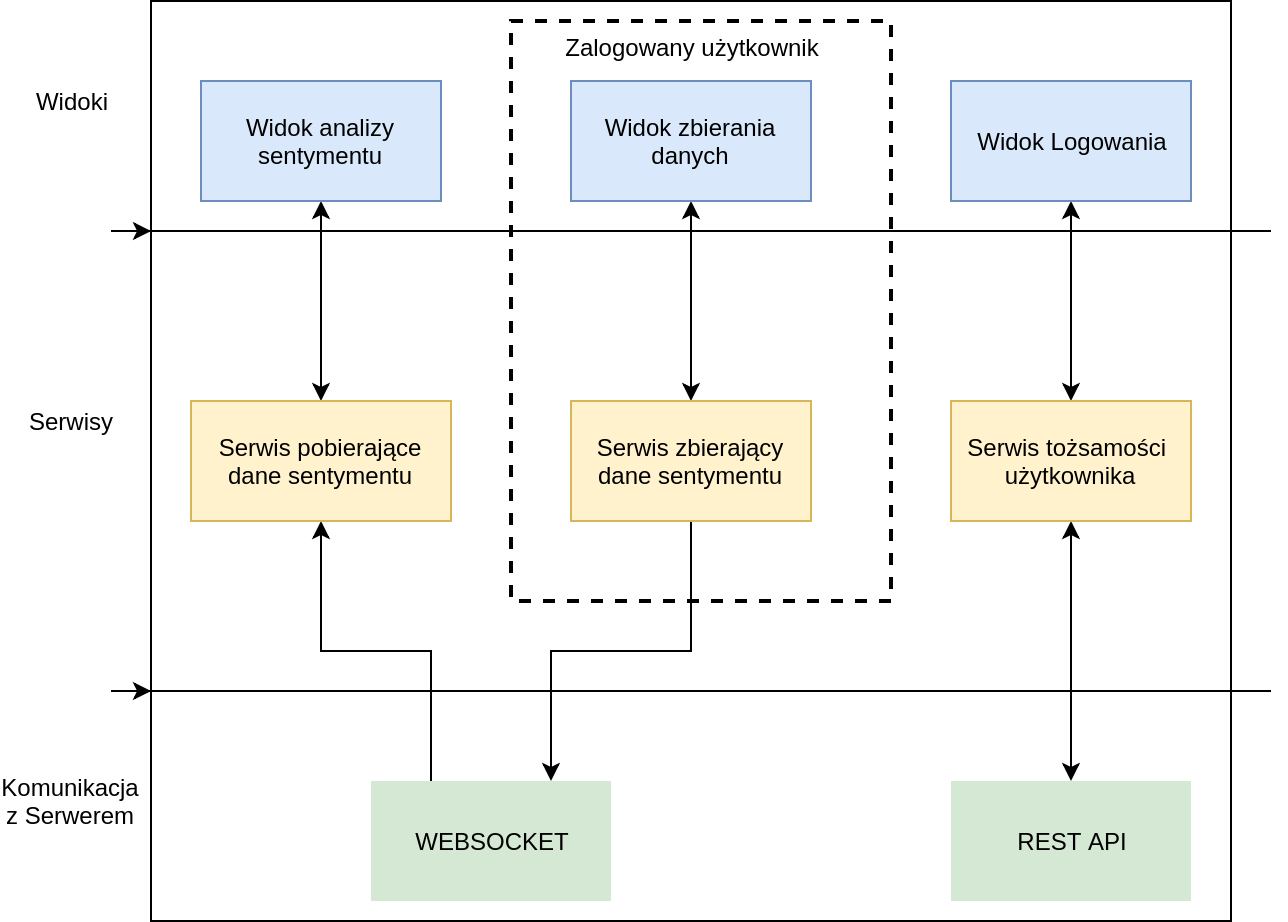
\includegraphics[width=0.95\textwidth]{img/client-modules.png}
  \caption{Diagram modułów klienta}
  \label{fig:client}
\end{figure}

\paragraph*{Widok analizy sentymentu}
\paragraph*{Widok logowania}
\paragraph*{Widok zbierania danych}
\paragraph*{Serwis pobierający dane sentymentu}
\paragraph*{Serwis zbierający dane sentymentu}
\paragraph*{Serwis tożsamości użytkownika}

\subsection{Technologie}
\subsubsection{Stack technologiczny}
\begin{itemize}
  \item {\textbf{aplikacja klienta}: Angular7}
  \item {\textbf{komunikacja klient-serwer}: WebSockets}
  \item {\textbf{serwer}: JavaEE}
  \item {\textbf{baza danych}: MongoDB}
\end{itemize}
\clearpage
\subsubsection{Wybrane technologie}
\begin{itemize}
    \item {\textbf{MongoDB} - jest nierelacyjnym systemem zarządzania bazą danych, który charakteryzuje się wysokiego stopnia skalowalności100%ą oraz brakiem jednolitej struktury obsługiwania baz danych. MongoDB składuje dokumenty w postaci plików JSON, które zwyczajowo nazywane są dokumentami i umieszczane są w tzw. kolekcjach. Silnik nie wymaga tworzenie schematu bazy danych - schemat działania opiera się na wstawianiu dokumentów w odpowiednie kolekcje. W przypadku, gdy dana kolekcja nie istnieje, zostaje ona automatycznie stworzona. W porównaniu z relacyjnymi bazami danych, MongoDB charakteryzuje się większą wydajnością oraz możliwością skalowania bazy na wiele serwerów.}
    \item {\textbf{Angular7} - z uwagi na dobrą integrację z TypeScriptem, który wprowadza typowanie do JS. TUTAJ MUSISZ POMÓC XD}
    \item {\textbf{WebSockets} - jest technologią zapewniającą dwukierunkowy (full duplex) kanał komunikacji. Charakteryzuje się mniejszym kosztem wymiany danych niż REST oraz większą skalowalnością horyzontalną - ingerencja w daną strukturę poprzez dodawanie bądź usuwanie kolejnych serwerów. Decyzja o wyborze ww. technologii została podjęta na podstawie charakteru tworzonej aplikacji - wysyłanie dużych porcji danych do serwera oraz przeglądanie danych pochodzących z wybranego przedziału czasowego.}
\end{itemize}

\begin{thebibliography}{9}
\bibitem{sentiment} 
Baker, Malcolm, and Jeffrey Wurgler. 2007. 
\textit{"Investor Sentiment in the Stock Market."}
 Journal of Economic Perspectives, 21 (2): 129-152.
\end{thebibliography}
\end{document}